% !TEX encoding = UTF-8 Unicode
\documentclass[a4paper, 12pt]{article}
\usepackage{graphicx}
\usepackage[brazil]{babel}
\usepackage[utf8]{inputenc}

\author{Seu nome}
\title{}

\linespread{1.5}


\begin{document}
%Capa
\begin{center}
\textbf{MINISTÉRIO DA DEFESA}\\
\textbf{EXÉRCITO BRASILEIRO}\\
\textbf{DEPARTAMENTO DE CIÊNCIA E TECNOLOGIA}\\
\textbf{INSTITUTO MILITAR DE ENGENHARIA}\\
\textbf{Seção de Engenharia de Sistemas / SE 8}

\vspace{2.5cm}

\begin{large}
\textbf{Proposta de Tema de Dissertação de Mestrado
\\Curso: Mestrado em Sistemas e Computação}

\vspace{1.5cm}

\textbf{Titulo de seu trabalho}

\vspace{1.5cm}


\textbf{Orientador: Nome do Orientador, Ph.D}

\end{large}

\vspace{1.5cm}

\textbf{Aluno: Seu nome (SC XXXXX)}


\vspace{2cm}

\begin{small}
Data de Apresentação no SE/8:\\
Rio de Janeiro, XX de mestal do ano tal
\end{small}

\end{center}


%Título
\newpage
\begin{large}
\section{Título da Dissertação}
\textbf{Título da Tese:}\\
\textbf{Titulo de sua tese}\\

\noindent\textbf{Título da Capa:}\\
\textbf{Titulo da capa}\\

\noindent\textbf{Área de Concentração:}\\
Tecnologias e Sistemas de Computação\\

\noindent\textbf{Linha de Pesquisa:}\\
Tecnologias para Tratamento e Transmissão da Informação\\
\end{large}

%Desenvolvimento do Texto
\newpage
\section{Introdução}
Em 2005, Lima \cite{TR:Sandro:05} e Botelho\cite{TR:Wagner:05} trabalharam no projeto de uma Casa Inteligente(trabalhos separados) com as seguintes características:
	\begin{itemize}
	\item Adaptação de suas condições internas com um mínimo de interferência dos moradores;
	\item O cômodo é adaptado de acordo com as preferências de temperatura ou luminosidade;
	\item Monitoração do consumo de energia;
	\item Medidas de segurança(detecção de invasores);
	\item Menos invasivo possível(sem uso de câmeras, microfones, painéis de controle);
\end{itemize}

Para a identificação dos indivíduos, Lima\cite{TR:Sandro:05} implementou um sensor de passos baseado em um tapete de células que detecta e retira três parâmetros dos passos: distância entre o passo, inclinação e frequência. Esses dados foram submetidos a uma rede neural a qual é responsável por classificar o indivíduo. A idéia de se implementar um sensor de passos, como sistema de identificação para a casa, foi essencial pois isso proporciona uma maneira não-invasiva de identificar os moradores, pois caminhar é um dos atos mais naturais em uma casa. A idéia do sensor de passos, sem dúvida, foi uma solução bem adequada para o problema de identificar os indivíduos. Porém, a implementação em uma casa real implicaria na substituição total, ou quase total, do piso da casa. 

Um outro sistema de identificação baseado no som dos passos, pode ser estudado de maneira que não alteraria a estrutura da residência. Alguns trabalhos na literatura\cite{TR:Shoji:04,TR:Shoji:05, TR:Itai:06} comprovaram que esta identificação é possível, pelo menos para um conjunto restrito executados nos testes.

Como o som é uma rica fonte de informação, além da identificação, é possível implementar um sistema de segurança no sentido de cuidar de pessoas idosas e/ou doentes, visto que pode se detectar a presença de gritos ou pancadas no ambiente. Isso contribui ainda mais para a escolha do som como alternativa para o sistema de identificação da casa. Este trabalho se propõe ao estudo de características contidas no som e através delas seja possível classificar os indivíduos.

\section{Objetivo}
Desenvolver um sistema de identificação para a Casa Inteligente, através da análise e extração de características do som produzido pelos passos dos indivíduos.

\section{Tarefas realizadas}
As tarefas realizadas nesse período se resumem nos seguintes tópicos:

\begin{itemize}
	\item Estudo das propriedades da marcha humana;
	\begin{itemize}
	\item Fases do passo e as etapas de cada fase;
	\item A identificação dessas fases na onda sonora;
	\end{itemize}
	\item Estudo de parâmetros objetivos do som;
	\begin{itemize}
	\item Medidas estatísticas:
	\begin{itemize}
		\item Momentos Espectrais;
		\item Skewness e kurtosis;
		\item Moda espectral;
	\end{itemize}
	\item Coeficientes Cepstrais e Mel-Cepstrais;
	\item Frequência dos passos;
	\item Coeficientes de Predição Linear;
	\item Grau de Similaridade do espectro;
\end{itemize}
	\item Elaboração de um banco de testes iniciais;
	\begin{itemize}
		\item Foi gravado o som de alguns indivíduos caminhando para realizar os testes iniciais;
	\end{itemize}
\end{itemize}

\section{Dificuldades encontradas}
Lista de dificuldades...
\section{Próximas etapas}
As próximas estapas se resumem a:
\begin{itemize}
	\item Escrever teste...
	\item Fazer apresentação em latex para o proximo período;
\end{itemize}

\section{Cronograma} \label{sec:crono}
Para facilitar a compreensão do projeto, optou-se por dividir o projeto em módulos que seguirão o cronograma abaixo.
\begin{figure}[h]
	\centering
		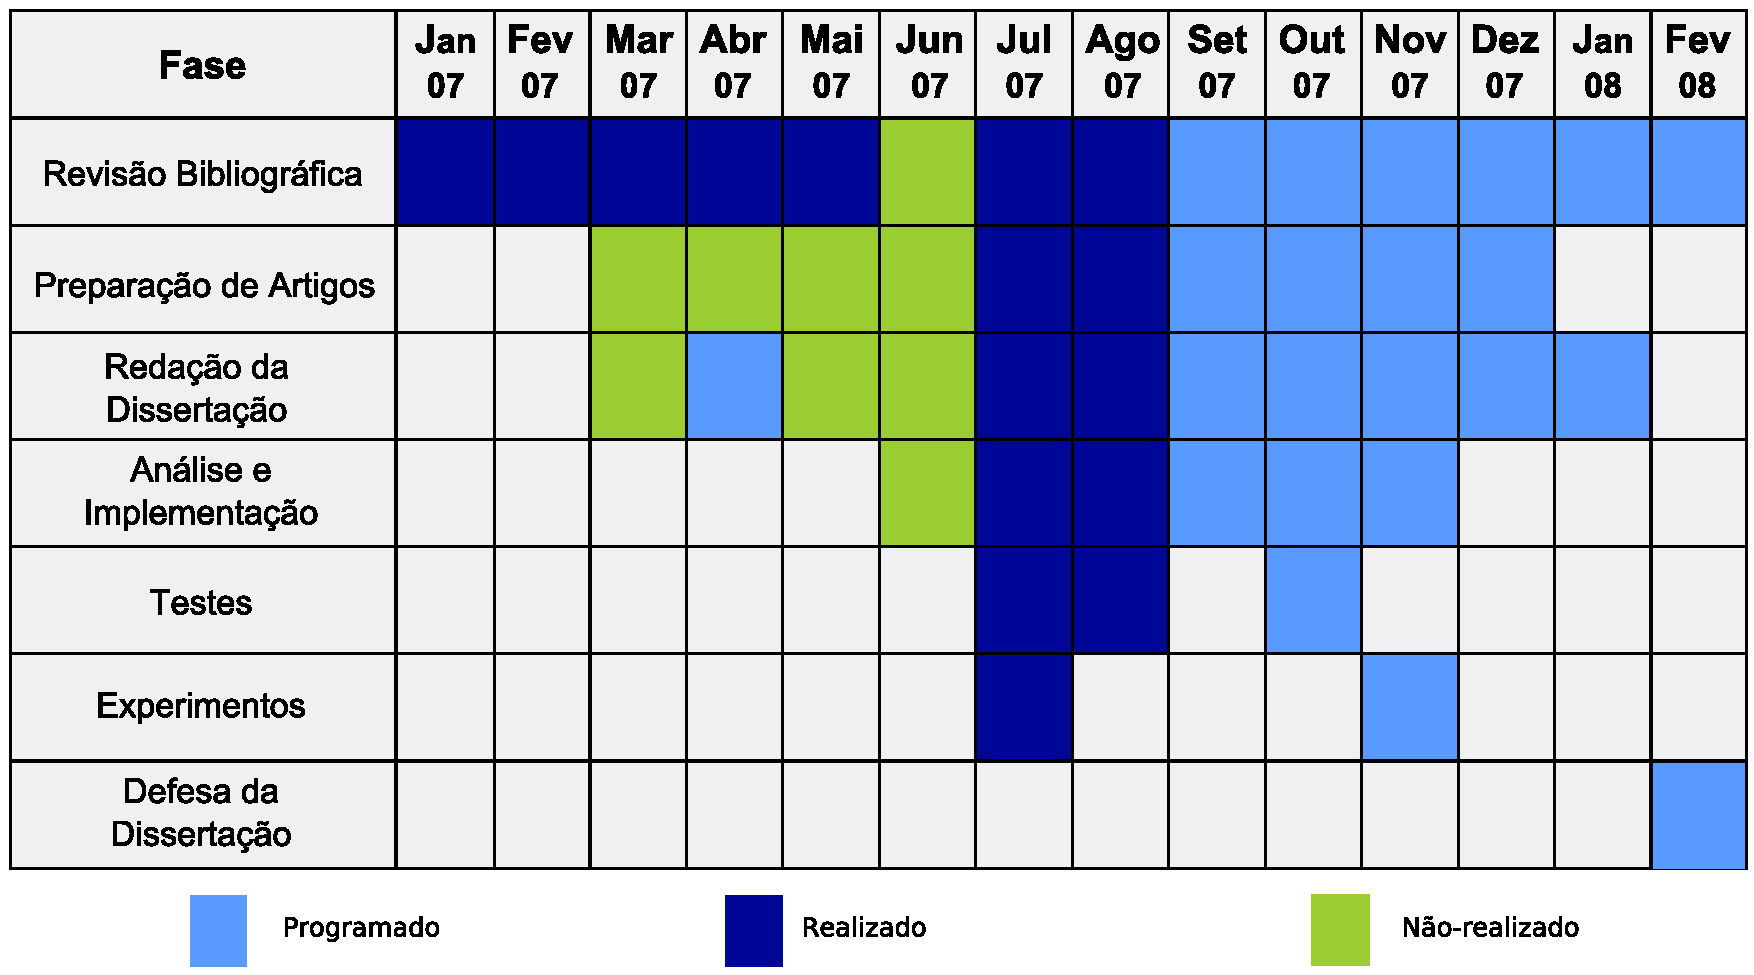
\includegraphics[scale=0.4]{img/cronograma.pdf}
	\caption{Cronograma físico.}
	\label{fig:cronograma}
\end{figure}

\bibliographystyle{abbrv}
\bibliography{ref} 

\newpage

\begin{center}
\_\_\_\_\_\_\_\_\_\_\_\_\_\_\_\_\_\_\_\_\_\_\_\_\_\_\_\_\_\_\_\_\_\_\_\_\_\_\_\_\_\_\_\_\_\_\_\_\_\_\_ \\

Seu Nome (SC XXX) \\Aluno \\ 
 
\hspace{4cm}
\\


\_\_\_\_\_\_\_\_\_\_\_\_\_\_\_\_\_\_\_\_\_\_\_\_\_\_\_\_\_\_\_\_\_\_\_\_\_\_\_\_\_\_\_\_\_\_\_\_\_\_\_ \\
Nome do orientador, Ph.D \\Orientador \\ 

\hspace{4cm}
\\


\_\_\_\_\_\_\_\_\_\_\_\_\_\_\_\_\_\_\_\_\_\_\_\_\_\_\_\_\_\_\_\_\_\_\_\_\_\_\_\_\_\_\_\_\_\_\_\_\_\_\_ \\
Maj Ronaldo Moreira Salles, Ph.D \\Coordenador de Pós-Graduação \\

\hspace{4cm}

\end{center}
Concordo com a presente Proposta de Dissertação e declaro que as necessidades para sua execução serão garantidas pelo departamento. \\
IME, em \today
 \hspace{4cm}
 \\
 \\
 \\
 \\
 
\begin{center}
\_\_\_\_\_\_\_\_\_\_\_\_\_\_\_\_\_\_\_\_\_\_\_\_\_\_\_\_\_\_\_\_\_\_\_\_\_\_\_\_\_\_\_\_\_\_\_\_\_\_\_\_\_\_\_\_\_\_\_ \\
Antonio Carlos Freire de Almeida, Ten Cel QEM, \\
CHEFE SE/8
\end{center}
\end{document}